\documentclass[12pt]{article} % use larger type; default would be 10pt
\usepackage[utf8]{inputenc} % set input encoding (not needed with XeLaTeX)
\usepackage{fancyhdr}


\usepackage{geometry, ulem, soul, color, graphicx, hyperref, array, caption, titling, enumerate} % to change the page dimensions
\geometry{letterpaper}
\usepackage[dvipsnames]{xcolor}
\usepackage{amsmath,amssymb}

 %put box around figure captions
\makeatletter
\long\def\@makecaption#1#2{%
  \vskip\abovecaptionskip
  \sbox\@tempboxa{\fbox{#1: #2}}%
  \ifdim \wd\@tempboxa >\hsize
    \fbox{\parbox{\dimexpr\linewidth-2\fboxsep-2\fboxrule}{#1: #2}}\par
  \else
    \global \@minipagefalse
    \hb@xt@\hsize{\hfil\box\@tempboxa\hfil}%
  \fi
  \vskip\belowcaptionskip}
\makeatother

\usepackage[compact]{titlesec}
\titlespacing{\section}{0pt}{*1}{*0}
\titlespacing{\subsection}{0pt}{*1}{*0}
\titlespacing{\subsubsection}{0pt}{*0}{*0}

\linespread{1.2}


\setlength\parindent{0pt}
\setlength\parskip{12pt}
\usepackage{float}
\geometry{margin=1in}

\DeclareMathOperator{\E}{\mathbb{E}}



\pagestyle{fancy}

\lhead{CS 155 Set 1}
\rhead{Timothy Liu}
\pagenumbering{arabic}



\title{CS155 Set 1}
\author{Timothy Liu}

\begin{document}


\maketitle

\newpage
\section{Problem 1}
\subsection{Part A}
A hypothesis set is the collection of possible candidates functions representing a model.

\subsection{Part B}
The hypothesis set of a linear model is a weight vector $w$ that has a selected number of dimensions (depending on the number of parameters we are fitting to) and a scalar $b$.

\subsection{Part C}
Overfitting is when the model fits too closely to the training set. Overfitting occurs when the in sample error is decreasing but the out of sample error increases.

\subsection{Part D}
One way of preventing overfitting is to increase the size of the training set. The second way is to use a simpler model with fewer parameters.

\subsection{Part E}
The training data is the data that you look at to construct you learning model. The model is ``trained" using the training data. The test data is a separate set of data that the learning algorithm is not trained on. Instead, the learning model, after being trained on the training data, is then applied on the test data to evaluate the model's performance. If you change the model based on the test set, then you are using the test set as the training set. Doing this will compromise the test set's ability to predict how well your model performs on out of sample data.

\subsection{Part F}
We assume that the dataset is sampled independently and identically. This means each dataset has the same distribution as other datasets and that they are independent of each other.

\subsection{Part G}
The input space $X$ is a set of emails and the output space $Y$ are labels that indicate if each email is either spam or not spam.

\subsection{Part H}
$k$-fold validation is a technique for estimating the out of sample error of an algorithm. In this technique, the original training data is broken into multiple partitions. One partition is set aside as the validation set, and the algorithm is trained on the other partitions. The trained algorithm is then evaluated on the untouched validation set. The process is repeated, and each partition is used as the validation set.

\section{Problem 2}

\subsection{Problem A}
$$ \E_s[E_{out}(f_s)] $$
Substitution
$$ \E_s[\E_x[(f_s(x) - y(x))^2]] $$
Swap order of expected value
$$ \E_x[\E_s[(f_s(x) - y(x))^2]] $$
Add zero
$$ \E_x[\E_s[(f_s(x) - F(x) + F(x) - y(x))^2]] $$
Expand
$$ \E_x[\E_s[(f_s(x) - F(x))^2 + (F(x) - y(x))^2 + 2(f_s(x) - F(x))(F(x) - y(x))]] $$
Expected value of cross term is zero
$$ \E_x[\E_s[(f_s(x) - F(x))^2 + (F(x) - y(x))^2 ]] $$
Linearity
$$ \E_x[\E_s[(f_s(x) - F(x))^2] + \E_s[(F(x) - y(x))^2 ]] $$
$$ \E_x[Bias(x)+ Var(x) ]] $$


\subsection{Problem B}

\begin{figure}[H]
	\makebox[\textwidth][c]{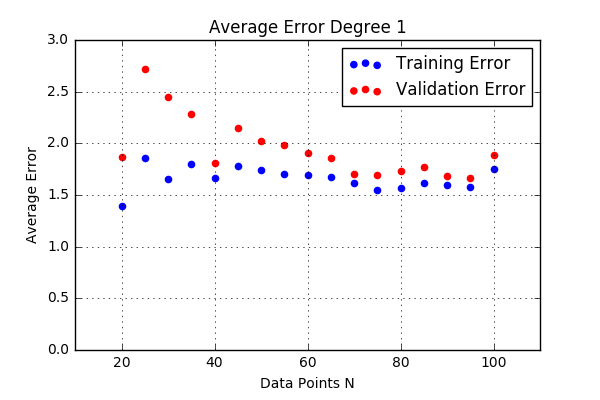
\includegraphics[width=5in]{p2_1.png}}
	\caption{Training and validation error for polynomial model degree 1.}
\end{figure}

\begin{figure}[H]
	\makebox[\textwidth][c]{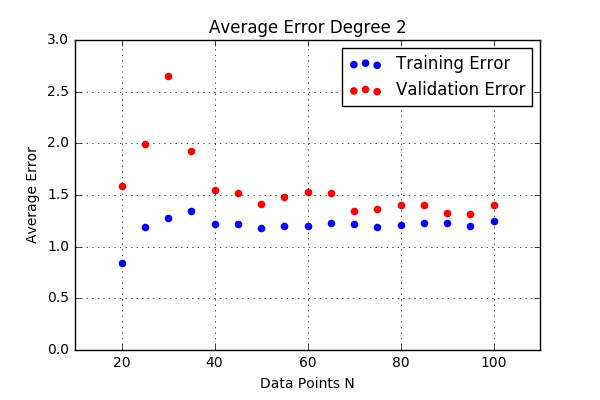
\includegraphics[width=5in]{p2_2.png}}
	\caption{Training and validation error for polynomial model degree 2.}

\end{figure}

\begin{figure}[H]
	\makebox[\textwidth][c]{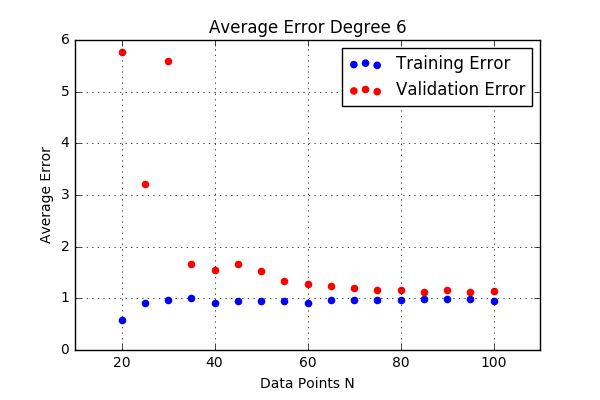
\includegraphics[width=5in]{p2_3.png}}
	\caption{Training and validation error for polynomial model degree 6.}

\end{figure}

\begin{figure}[H]
	\makebox[\textwidth][c]{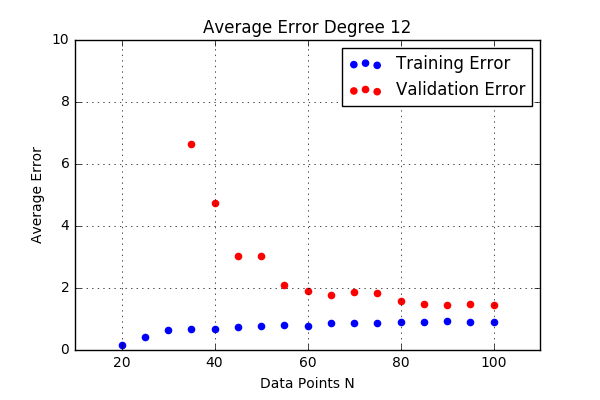
\includegraphics[width=5in]{p2_4.png}}
	\caption{Training and validation error for polynomial model degree 12. Some validation 	errors are not shown because their value greatly exceeds that of the other points.}

\end{figure}

\subsection{Problem C}
The 1-degree model has the highest bias. This model has an average training error of about 1.6 to 1.7 regardless of the size of the training set, which is the highest of the four models. Models with lower complexity also generally have more bias.

\subsection{Problem D}
The 12-degree model has the largest variance. The validation error for this model is the highest, and for a small training set the validation error is many orders of magnitude greater than that of the other models.

\subsection{Problem E}
The quadratic model may improve slightly but not greatly if we included more training points. After roughly 70 points the average validation error is fairly stable, suggesting that adding more points won't necessarily lead to improved performance.

\subsection{Problem F}
The training error is generally lower because the models are optimized to minimize the error of the points in the training set. Since the points from the validation set are not used to help create the model, the validation error is generally greater.

\subsection{Problem G}
The 6 degree model trained on the most number of points possible will perform the best on out-of-sample data. This model has the lowest validation error - slightly greater than 1 - and the validation error is an approximate indicator of how well the model will perform on unseen data.

\section{Problem 3}

\subsection{Problem A}

\begin{figure}[H]
	\makebox[\textwidth][c]{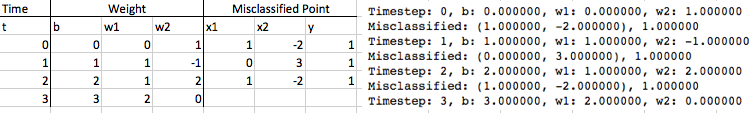
\includegraphics[width=7in]{p3_1.png}}
	\caption{Weights of perceptron at each timestep and misclassified point.}
\end{figure}

\subsection{Problem B}
In 2D the smallest non-linearly-separable  data set has 4 points. If there are 3 points, then if two points are classified the same then a line can be drawn between the third point and the two similarly classified point. If there are 4 points,  3 points can be classified +1 and arranged in a triangle. If the fourth point is labeled -1 and placed at the center of the triangle, the data is not linearly separable.

Similarly, for a 3D dataset the smallest non-linearly-separable data set has 5 points. 4 points can be arranged in a tetrahedron and classified +1, and the fifth point is in the middle of the tetrahedron and classified -1. Any dataset with 4 points can be linearly separated in 3D, since a plane can be drawn between 3 points similarly classified and then shifted slightly towards the fourth, differently classified point.

For an N-dimensional set, the smallest non-linearly separable set has N+2 points.

\subsection{Problem C}
\vspace{-5mm}

\begin{figure}[H]
	\makebox[\textwidth][c]{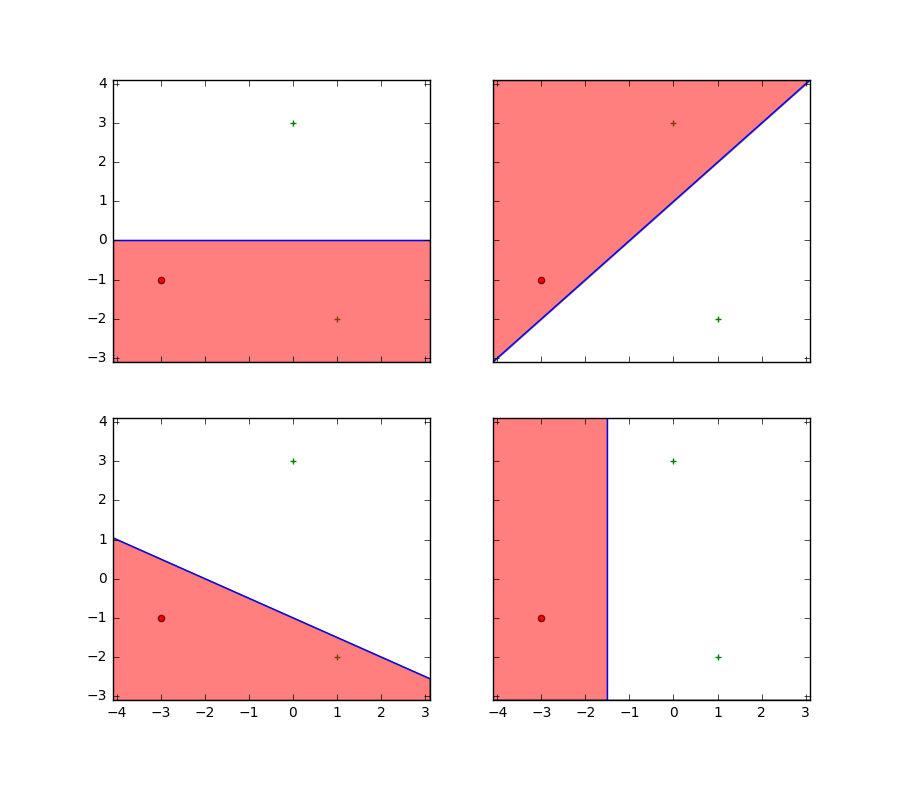
\includegraphics[width=4in]{separable.png}}
	\vspace{-15mm}
	\caption{Visualization of data set from part A.}
\end{figure}
\vspace{-5mm}
\begin{figure}[H]
	\makebox[\textwidth][c]{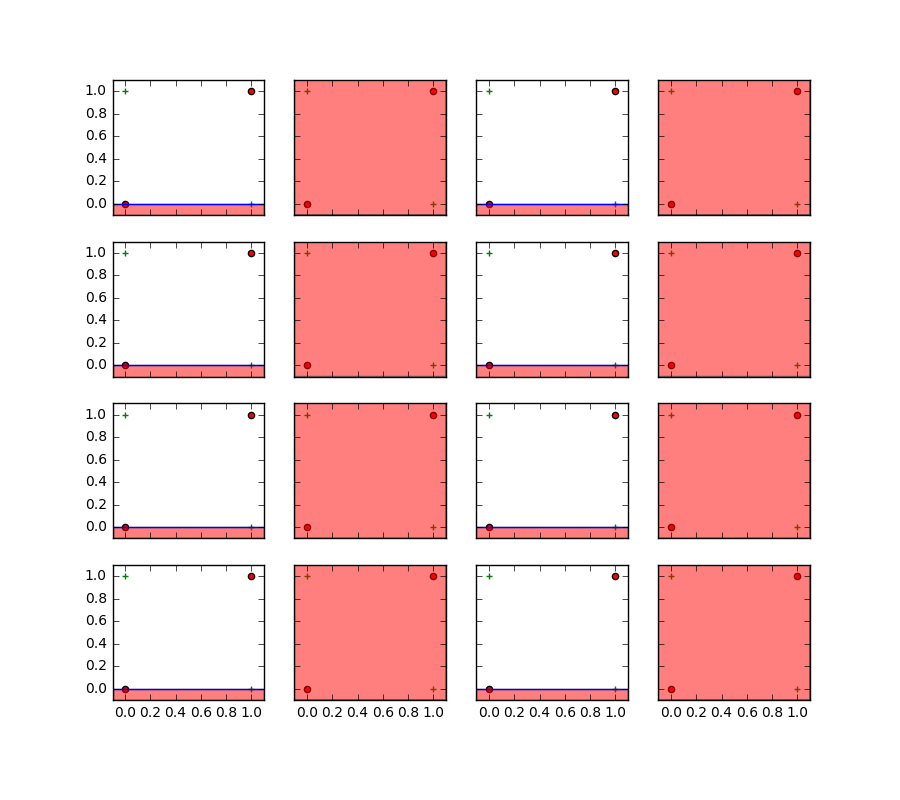
\includegraphics[width=4in]{non-separable.png}}
	\vspace{-15mm}
	\caption{Visualization of non-separable data set.}
\end{figure}

If the dataset is not linearly separable, then the PLA will never converge. As demonstrated in the graph above, the PLA will oscillate between two solutions, each of which misclassifies a different point. Updating the weights to correctly classify one solution will lead to the other solution being misclassified.

\section{Problem 4}
\subsection{Problem A}
We define a zeroth coordinate for the weight vector \textbf{w} and for each training point \textbf{x}. Every former \textbf{x} = $(x_1, x_2, x_3.....)$ is instead $(1, x_1, x_2, x_3.....)$ and the weight vector now includes a $w_0$ term: $(w_0, w_1, w_2.....)$. The $w_0$ is the bias term, and the relation between $w_0$ and b is $w_0 = b \div i$

\subsection{Problem B}
We want the derivative of the squared loss function for linear regression with respect to the vector \textbf{w}.

$$\partial _w \sum_{i = 1}^{N} (y_i - \textbf{w}^T\textbf{x}_i)^2$$
$$\sum_{i = 1}^{N} \partial _w (y_i - \textbf{w}^T\textbf{x}_i)^2$$
$$\sum_{i = 1}^{N} 2 * (y_i - \textbf{w}^T\textbf{x}_i) \partial _w (y_i - \textbf{w}^T\textbf{x}_i)$$
$$\sum_{i = 1}^{N} -2 * (y_i - \textbf{w}^T\textbf{x}_i) \textbf{x}_i$$

\subsection{Problem C}
See src.



\subsection{Problem D}
As the starting point is changed, the weights take a different path to convergence but they reach the same minimum. The starting point has some influence on how quickly the weights converge, though it seems like they all converge about as quickly. Dataset 2 has certain points that converge more quickly than others.

\subsection{Problem E}

\begin{figure}[H]
	\makebox[\textwidth][c]{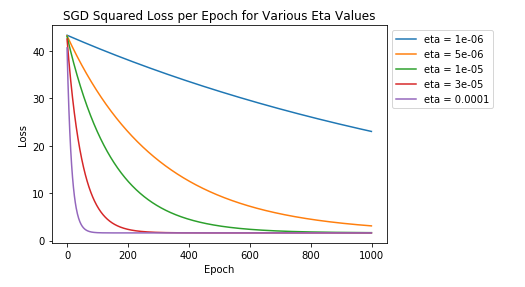
\includegraphics[width=4in]{DifferentEta.png}}
	\vspace{-15mm}
	\caption{Visualization of non-separable data set.}
\end{figure}

The squared loss falls much more rapidly for a larger eta. A larger eta leads to a faster convergence to a solution.
 






\end{document}
